% !TEX root = ../main.tex

We have implemented all aspects of our approach in $\mathtt{vigir\_behavior\_synthesis}$,\footnote{\scriptsize{\url{https://github.com/team-vigir/vigir_behavior_synthesis}}}
 a collection of Robot Operating System (ROS) Python packages.
Figure \ref{Fig:vigir_behavior_synthesis} depicts these packages as well as the nominal workflow.

\begin{figure}[t]
\centering
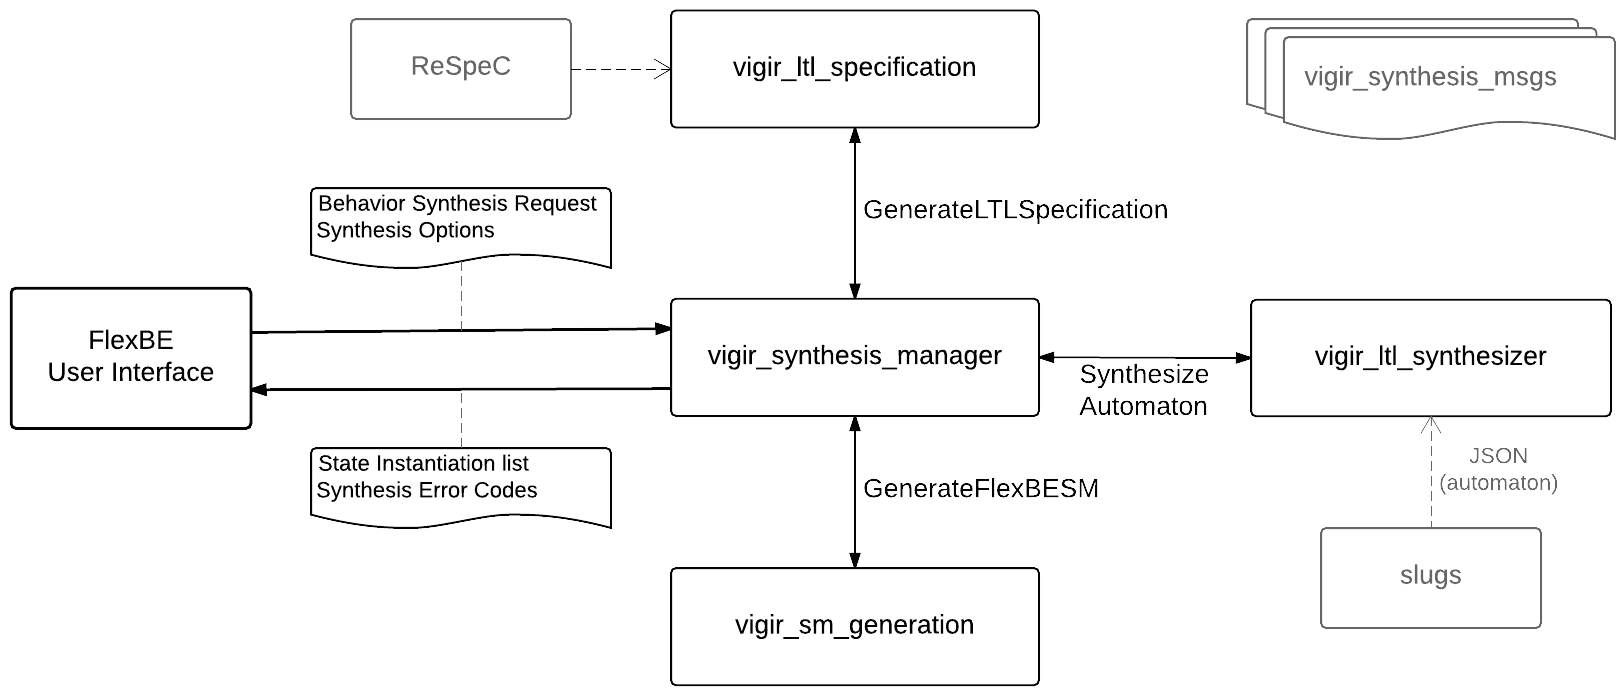
\includegraphics[width=0.99\columnwidth,clip]{./img/behavior_synthesis_packages.png}
\caption{
	Team ViGIR's ``Behavior Synthesis" ROS packages and the nominal workflow (clockwise, starting from the left).
}
\label{Fig:vigir_behavior_synthesis}
\end{figure}

The synthesis action server ($\mathtt{vigir\_synthesis\_manager}$) receives a request from the user via FlexBE's GUI.
Given the user's input (initial conditions and goals), the server first requests a full set of \textsc{ltl} formulas for Atlas from the $\mathtt{Generate LTL Specification}$ service ($\mathtt{vigir\_ltl\_specification}$ package).
The generation of the \textsc{ltl} formulas from Section \ref{S:ltl} is delegated to our ``Reactive Specification Construction kit" (ReSpeC),\footnote{\scriptsize{\url{https://github.com/team-vigir/ReSpeC}}}
 which is a Python framework with rudimentary ROS integration.

\begin{figure}[t]
\centering
\fbox{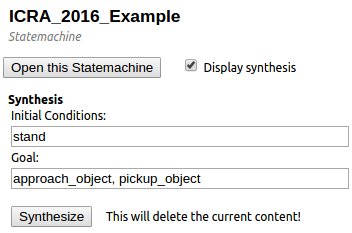
\includegraphics[width=0.90\columnwidth,clip]{./img/synthesis_menu_simple.png}}
\caption{Screenshot of the FlexBE Editor's synthesis menu.
	\todo[inline, caption = {Safer synthesis menu example}]{This is a risky example because a reviewer might say ``Why does the user have to explicitly tell the robot to approach the object before picking it up?"}
}
\label{Fig:SynthesisMenuSimple}
\end{figure}

The $\mathtt{vigir\_ltl\_synthesizer}$ package acts as a wrapper for external synthesis tools (currently, \cite{SLUGS} is supported).
Given the generated \textsc{ltl} specification, the $\mathtt{Synthesize Automaton}$ service returns a finite-state automaton that is guaranteed to satisfy it, if one exists.
Finally, the server requests a $\mathtt{State Instantiation}$ message from the $\mathtt{Generate FlexBE SM}$ service ($\mathtt{vigir\_sm\_generation}$ package).
This message provides the FlexBE Editor with sufficient information to generate Python code, i.e., an executable state machine that instantiates the synthesized automaton.
The corresponding action, services, and messages are defined in the $\mathtt{vigir\_synthesis\_msgs}$ package.

%\begin{algorithm}[t]
The following excerpt\footnote{We have omitted some details for the sake of brevity and clarity of presentation. For example, most list elements are strings, e.g., \scriptsize{\texttt{"template\_id"}}.}
 is taken from the $\mathtt{State Instantiation}$ list message, which is the end product of the $\mathtt{vigir\_behavior\_synthesis}$ workflow (Fig. \ref{Fig:vigir_behavior_synthesis}).
Specifically, this excerpt corresponds to the primitive functionality $\mathtt{object\_template}$, which appears in Fig. \ref{Fig:stand_and_pick_sm}.

\begin{description}
\setlength{\itemindent}{-.4in}
	\item \scriptsize{\texttt{state\_path: /4\_object\_template}}
	\item \scriptsize{\texttt{state\_class: InputState}}
	\item \scriptsize{\texttt{parameter\_names: [request]}}
	\item \scriptsize{\texttt{parameter\_values: [InputState.SELECTED\_OBJECT\_ID]}}
	\item \scriptsize{\texttt{outcomes: [no\_connection, aborted, received, data\_error]}}
	\item \scriptsize{\texttt{transitions: [failed, failed, 6\_manipulate, failed]}}
	\item \scriptsize{\texttt{autonomy: [0, 0, 0, 0]}}
	\item \scriptsize{\texttt{userdata\_keys: [data]}}
	\item \scriptsize{\texttt{userdata\_remapping: [template\_id]}}
\end{description}

%\caption{Excerpt from $\mathtt{State Instantiation}$ message}
%\label{Alg:StateInstantiation}
%\end{algorithm}

% END